\documentclass[10pt]{article}

% ---------- Layout: two-column journal style, matching sample.pdf ----------
\usepackage[a4paper,margin=1.9cm,columnsep=0.7cm]{geometry}
\usepackage{multicol}
\usepackage{graphicx}
\usepackage{amsmath,amssymb}
\usepackage{booktabs}
\usepackage{tikz}
\usetikzlibrary{arrows.meta,positioning,fit,backgrounds}
\usepackage{fancyhdr}
\usepackage{enumitem}
\usepackage[hidelinks]{hyperref}
\usepackage{caption}
\usepackage{titlesec}
\usepackage{xcolor}

\setlength{\parindent}{0pt}
\setlength{\parskip}{0.4em}

\titleformat{\section}{\normalfont\large\bfseries}{\thesection.}{0.5em}{}
\titleformat{\subsection}{\normalfont\bfseries}{\thesubsection}{0.5em}{}
\titlespacing*{\section}{0pt}{1.1em}{0.5em}
\titlespacing*{\subsection}{0pt}{0.9em}{0.4em}

\pagestyle{fancy}
\fancyhf{}
\fancyhead[L]{\footnotesize Ledger N3XT Student Research \, --- \, Privacy Track}
\fancyhead[R]{\footnotesize \thepage}
\renewcommand{\headrulewidth}{0.4pt}

\captionsetup{font=small,labelfont=bf}

\newcommand{\papertitle}{The Custody--Privacy Gap: What a Ten-Dollar Hardware Wallet Reveals About Self-Custody on Public Ledgers}
\newcommand{\paperauthor}{Arnav Panjla\textsuperscript{1} \, and \, Sahitya Shankar\textsuperscript{1}}
\newcommand{\paperaffil}{\textsuperscript{1}Blockchain Society, IIT Delhi}
\newcommand{\paperemail}{arnavpanjla@gmail.com, yraretil@gmail.com}

\begin{document}

% ---------------- Title block (single column, matches sample.pdf layout) ----------------
\twocolumn[
  \begin{@twocolumnfalse}
    \begin{center}
      {\LARGE \bfseries \papertitle \par}
      \vspace{0.6em}
      {\large \paperauthor \par}
      {\small \paperaffil \\ \texttt{\paperemail} \par}
      \vspace{1.0em}
    \end{center}
    \noindent\rule{\textwidth}{0.6pt}
    \vspace{0.6em}

    \textbf{Abstract.} Every self-custody hardware wallet is sold on one promise: your private key never leaves the device. Noir Wallet, a \$10 open-source hardware-wallet prototype built on a \$3--5 STM32F401CCU6 microcontroller (WeAct BlackPill board) and a \$1--\$2 ATECC608A secure element, is used here as a working hardware case study and an incomplete signer design. V0 demonstrates the display, buttons, USB enumeration, hardware-random command path, BIP-39 generation, and Ethereum address derivation; transaction ingestion, PIN gating, and secure-element-backed secp256k1 signing are not implemented. We model the intended signing pipeline stage by stage --- secure element, firmware, USB HID transport, host software, broadcast node, public ledger --- and show that even perfect hardware-anchored key custody would leave every later stage observable. Address reuse, transaction-graph clustering, and host-side metadata survive perfect key custody untouched. We use a real bring-up bug found on this device, a secure element whose random number generator produces a fixed diagnostic pattern until its configuration zone is permanently locked, as a concrete illustration of what a verifiable hardware security claim looks like. We then map where privacy-enhancing techniques such as stealth addresses, zero-knowledge proofs of authorization, and selectively disclosable credentials would need to sit on top of this hardware to close the gap.

    \textit{Keywords:} self-custody, secure elements, hardware wallets, zero-knowledge proofs, transaction privacy, chain surveillance, ATECC608A

    \vspace{0.8em}
    \noindent\rule{\textwidth}{0.6pt}
    \vspace{0.4em}
  \end{@twocolumnfalse}
]

% ==================================================================
\section{Introduction}

Public ledgers make ownership pseudonymous and the flow of funds globally visible \cite{meiklejohn2013}. A hardware wallet solves a narrower problem: it keeps the signing key off a compromised host. It says nothing about the transaction after it is signed. Marketing copy, and sometimes users, treat ``self-custody'' and ``private'' as synonyms. They are not. A hardware-signed payment from a reused address is as clusterable as one signed in a browser. The hardware protects the key, not what the key signs or where the signed artifact travels.

We investigate this gap using Noir Wallet, an open-source Ethereum hardware wallet built on an STM32F4 (WeAct BlackPill, ARM Cortex-M4F) for roughly \$10, as a concrete substrate rather than a hypothetical one. Using its firmware, its secure element, and a real bring-up bug, we ask: (1) where a hardware-wallet pipeline leaks privacy, (2) what a secure element can verifiably guarantee, and (3) whether the cost of a hardware root of trust is why privacy-preserving self-custody stays out of reach. Section~6 is the cost point. Section~5 compares this prototype to published Ledger and Trezor architectures on two physical attacks the \$10 build does not close.

\section{Background}

Address-reuse and multi-input clustering collapse pseudonyms into real-world clusters without breaking any cryptography \cite{meiklejohn2013}. The same class of heuristic applies to Ethereum through reuse and interaction graphs. Three primitives sit above a hardware signer, and only their cost on 64~KB SRAM matters here. ERC-5564 stealth addresses need elliptic-curve derivation, which this MCU already does \cite{erc5564}. Selective disclosure (W3C credentials / SD-JWT) lets a holder prove one claim without dumping the rest \cite{sdjwt2025}. Full zk-SNARK shielding, as in Zerocash, hides origin, destination, and amount \cite{zerocash2014} --- and needs working memory this board does not have (Section~7). OFAC's 2022 Tornado Cash action is why this paper treats selective disclosure as the more defensible near-term layer \cite{ofac2022}.

\section{Methodology}

This is a design-analysis paper, not a controlled lab experiment. The method is a structured architectural review of Noir Wallet's signing pipeline, firmware, and secure-element behavior, plus a comparison to published commercial architectures, in four steps:

\begin{enumerate}[leftmargin=1.3em,itemsep=0.15em]
  \item \textbf{Decompose} the intended signing pipeline into discrete stages, from key generation and derivation to broadcast on the public chain.
  \item \textbf{Classify} each stage's exposure: what an on-path or on-chain observer can see at that stage, independent of whether the key itself is ever compromised.
  \item \textbf{Measure} the unlocked ATECC608A \texttt{Random} output as a Shannon-entropy object (Section~4.3), using the documented diagnostic stream rather than a claimed post-lock capture. Configuration lock is one-way; this build has not been locked.
  \item \textbf{Compare} the same pipeline against published Ledger and Trezor hardware designs (Section~5), then map remaining leaks to protocol-layer mitigations (Section~7).
\end{enumerate}

The object of the model is the custody/privacy split, not key extraction --- the threat hardware wallets are already sold against.

\section{Case Study: Noir Wallet}

\subsection{Architecture}
Noir Wallet V0 runs on an STM32F401CCU6 microcontroller (WeAct BlackPill board, ARM Cortex-M4F at 84~MHz, 64~KB SRAM, 256~KB flash). It drives a 128$\times$64 OLED and five buttons, enumerates over USB HID, requests randomness and identity from an ATECC608A, generates a BIP-39 mnemonic, and derives an Ethereum address on the MCU. Incoming HID frames are currently discarded; no transaction parser, PIN gate, or production signing flow is complete. The ATECC608A does not hold the secp256k1 wallet key. Figure~\ref{fig:arch} shows the physical layout; Figures~\ref{fig:cad}--\ref{fig:opencase} show the build.

\begin{figure}[t]
  \centering
  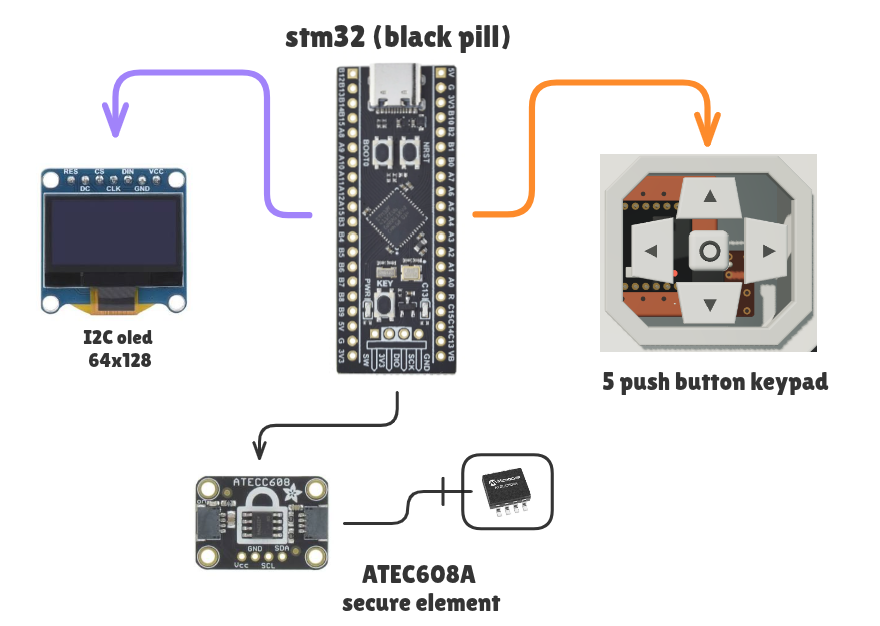
\includegraphics[width=0.95\linewidth]{images/architecture_schematic.png}
  \caption{Noir Wallet hardware layout: STM32F401CCU6 MCU (BlackPill), SSD1306 OLED, ATECC608A secure element, and push-button input, all on a single I\textsuperscript{2}C/GPIO bus.}
  \label{fig:arch}
\end{figure}

\begin{figure}[t]
  \centering
  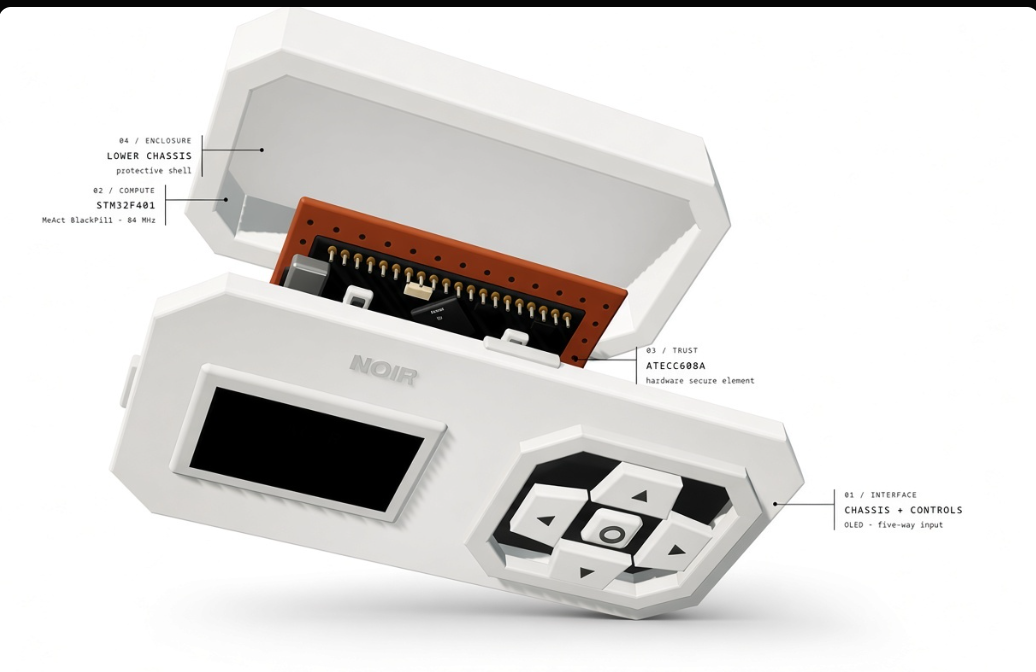
\includegraphics[width=0.85\linewidth]{images/CAD.png}
  \caption{Enclosure CAD model.}
  \label{fig:cad}
\end{figure}

\begin{figure}[t]
  \centering
  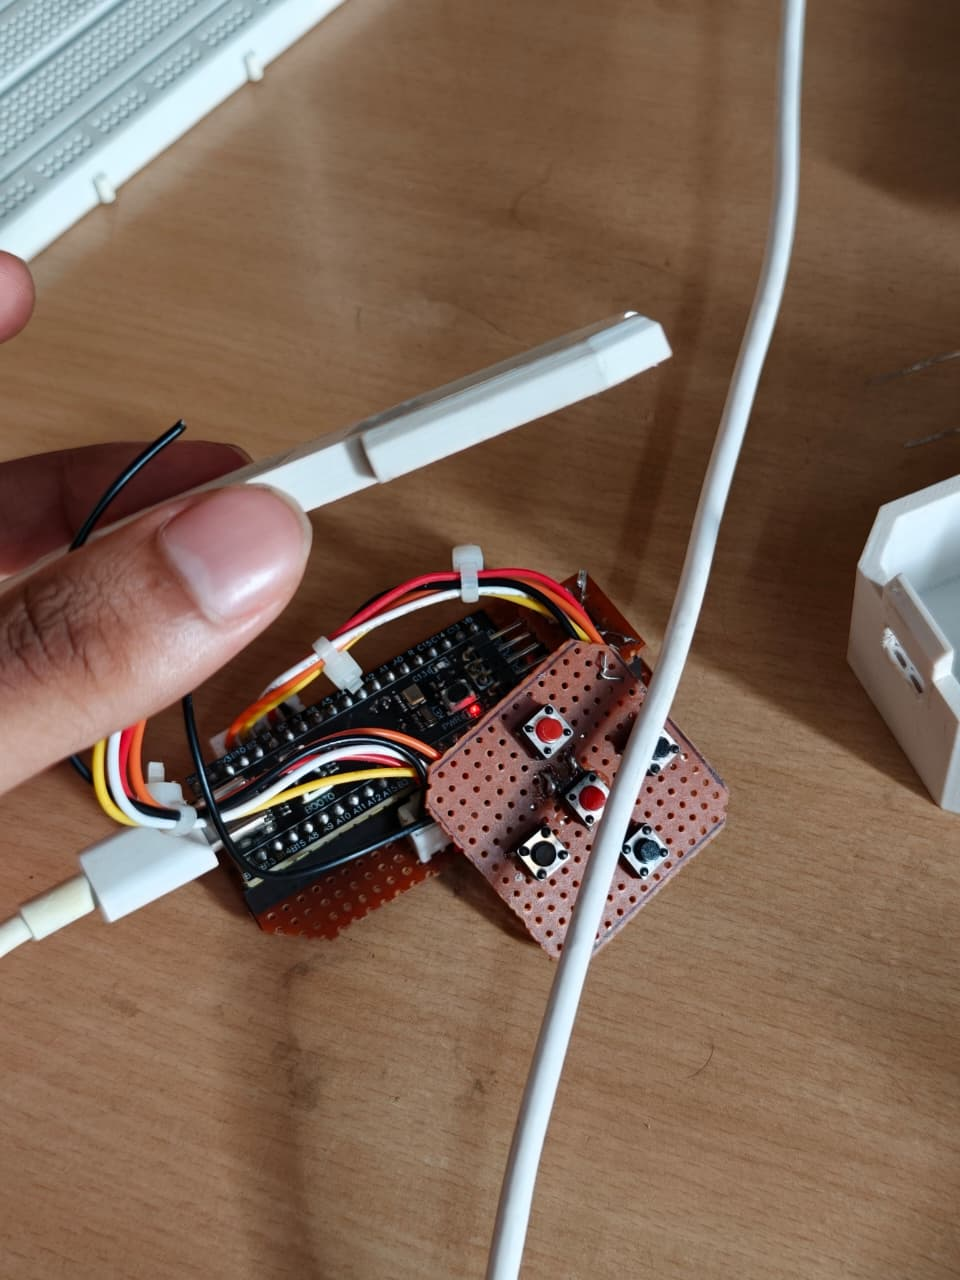
\includegraphics[width=0.85\linewidth]{images/device_internals.jpeg}
  \caption{Assembled internals: STM32F401CCU6, button matrix, OLED header.}
  \label{fig:internals}
\end{figure}

\begin{figure}[t]
  \centering
  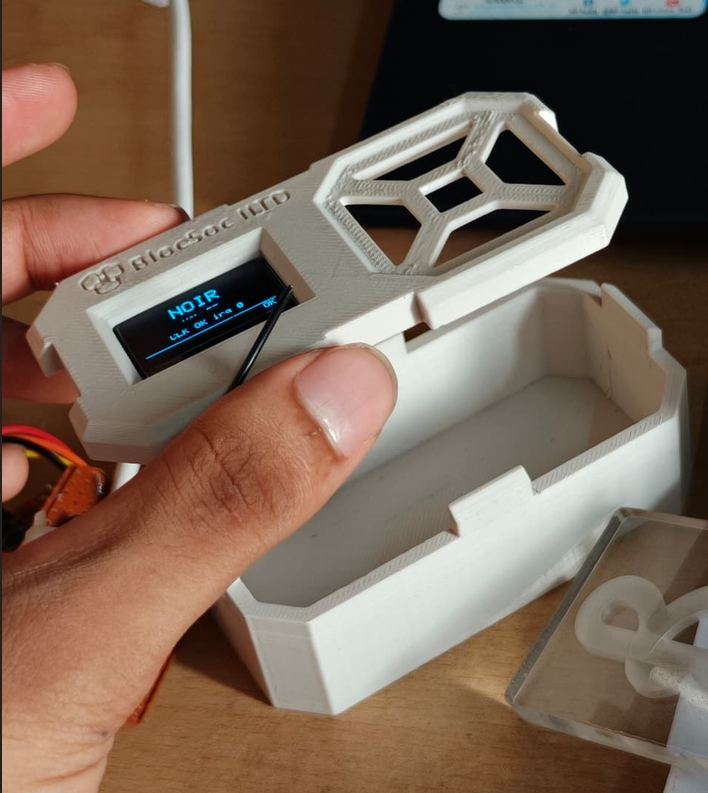
\includegraphics[width=0.75\linewidth]{images/device_open_case.png}
  \caption{The open enclosure with OLED powered on, showing the physical arrangement referenced throughout Section~4.}
  \label{fig:opencase}
\end{figure}

\subsection{What the secure element actually guarantees}
The ATECC608A is not a generic EEPROM; it is a cryptographic co-processor with hardware-enforced primitives \cite{atecc608a2019}. The following are chip capabilities, not claims that V0 uses them all; current firmware uses the random and serial commands:

\begin{itemize}[leftmargin=1.1em,itemsep=0.15em]
  \item \textbf{Non-exportable key storage} across 16 slots: a private key generated inside the chip can sign and derive, but the raw key material is never returned over the bus.
  \item \textbf{Hardware ECDSA/ECDH} on NIST P-256. This cannot directly sign Ethereum's secp256k1 transactions.
  \item \textbf{Hardware SHA-256/HMAC}, usable for firmware or command authentication independent of the MCU's own (much weaker) software stack.
  \item \textbf{An on-chip TRNG} specified against NIST SP~800-90A/B/C, with runtime health testing of the entropy source.
  \item \textbf{Monotonic counters and a one-way configuration lock}, which is the mechanism Section~4.3 turns into a worked example.
\end{itemize}

These capabilities are independently testable when configured and used. A claim like ``a P-256 private key generated in this slot is non-exportable'' can be checked against commands and bus traces. Noir V0 cannot yet make the same claim for its Ethereum secp256k1 key, which is derived transiently on the STM32.

\subsection{A worked example: the TRNG that wasn't random}
While bringing up this exact chip, we found that on an unconfigured, unlocked ATECC608A, the \texttt{Random} command (opcode \texttt{0x1B}) does not return entropy at all: it returns a fixed diagnostic pattern (\texttt{FF FF 00 00\ldots}), by design, to make bring-up testing deterministic. Microchip confirms this behavior applies until the configuration zone is permanently locked. On this unit it produced a fixed 12-word BIP-39 mnemonic every time, since the ``random'' seed was not random. The fix is a single one-way command, \texttt{Lock} (\texttt{0x17}, mode \texttt{0x80}) on the configuration zone, after which the same command returns genuine entropy.

This is offered deliberately as a small, unglamorous bug rather than a success story. It illustrates exactly what ``hardware-anchored trust'' should mean in a paper rather than a datasheet: a property that can fail silently, that failed in a specific, reproducible, and now-documented way on this device, and that has a specific, verifiable fix. The current shipped firmware still uses a demo-grade entropy backstop (an MCU cycle-counter XOR) rather than the locked TRNG, and this is stated plainly rather than papered over: it is not a NIST-certified source. A paper making unfalsifiable security claims about its own hardware would be exactly the kind of assertion this section argues against.

\paragraph{Making ``random'' measurable.} The bug is also why RNG claims need a repeated-invocation metric. Treated as one 32-byte draw, the pattern \texttt{FF FF 00 00\ldots} still contains two symbols and can look ``mixed.'' Across calls it does not: every invocation returns the same string, so the Shannon entropy of any fixed byte offset is $H = -\sum_i p_i \log_2 p_i = 0$ bits. Concatenating the documented diagnostic stream into 10{,}000 bytes yields only the symbols \texttt{0x00} and \texttt{0xFF} at equal frequency, so within-stream entropy is exactly $1.00$ bit/byte. An ideal IID uniform byte source sits at $8$ bits/byte. Figure~\ref{fig:entropy} plots those three numbers. The right-hand bar is a theoretical ceiling, not a measured post-lock capture: lock is one-way, and this firmware has not taken that step. NIST SP~800-90B's Repetition Count Test and Adaptive Proportion Test are built to catch exactly this class of stuck source \cite{nist80090b}.

\begin{figure}[t]
  \centering
  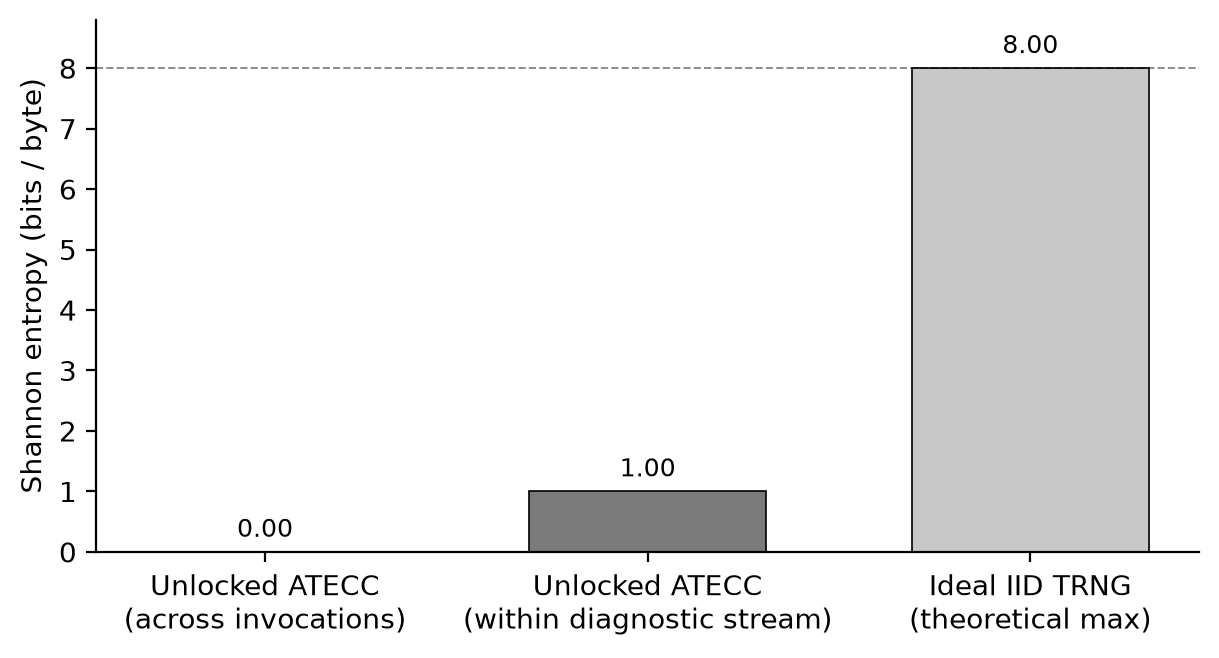
\includegraphics[width=0.95\linewidth]{images/entropy_shannon.png}
  \caption{Shannon entropy of the unlocked ATECC608A diagnostic RNG versus the 8-bit/byte ceiling of an ideal IID byte source. Left and center bars are computed from the documented \texttt{FF FF 00 00} stream (10{,}000 concatenated bytes). The right bar is theoretical, not a locked-device measurement.}
  \label{fig:entropy}
\end{figure}

\subsection{Where privacy actually leaks}
Figure~\ref{fig:leak} models the intended V1 pipeline for information exposure, not current V0 execution. If the signing key moves into a compatible secure element, that stage becomes dark while firmware, USB host, RPC node, and public ledger remain observable. V0 has not implemented the complete transaction path.

\begin{figure}[t]
  \centering
  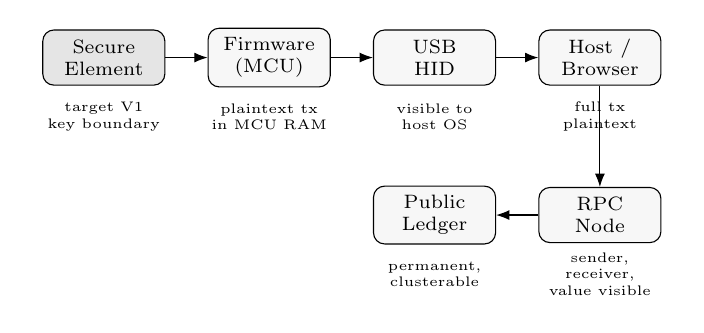
\begin{tikzpicture}[
      box/.style={draw, rounded corners, align=center, font=\scriptsize, minimum height=0.7cm, minimum width=1.55cm, fill=black!3},
      lock/.style={box, fill=black!10},
      lbl/.style={font=\tiny, align=center, text width=1.7cm},
      >=Latex
    ]
    % top row: signing pipeline, left to right
    \node[lock]                 (se)   at (0,0)    {Secure\\Element};
    \node[box]                  (fw)   at (2.1,0)  {Firmware\\(MCU)};
    \node[box]                  (usb)  at (4.2,0)  {USB\\HID};
    \node[box]                  (host) at (6.3,0)  {Host /\\Browser};
    % bottom row: post-broadcast, right to left under host/usb
    \node[box]                  (rpc)   at (6.3,-2.0) {RPC\\Node};
    \node[box]                  (chain) at (4.2,-2.0) {Public\\Ledger};

    \draw[->] (se) -- (fw);
    \draw[->] (fw) -- (usb);
    \draw[->] (usb) -- (host);
    \draw[->] (host) -- (rpc);
    \draw[->] (rpc) -- (chain);

    \node[lbl] at (0,-0.75)   {target V1\\key boundary};
    \node[lbl] at (2.1,-0.75) {plaintext tx\\in MCU RAM};
    \node[lbl] at (4.2,-0.75) {visible to\\host OS};
    \node[lbl] at (6.3,-0.75) {full tx\\plaintext};
    \node[lbl] at (6.3,-2.75) {sender, receiver,\\value visible};
    \node[lbl] at (4.2,-2.75) {permanent,\\clusterable};
  \end{tikzpicture}
  \caption{Modeled exposure across the intended signing pipeline. V0 does not yet implement this complete flow or secure-element-backed secp256k1 signing.}
  \label{fig:leak}
\end{figure}

PIN gating and offline signing would improve custody, but would not stop the host from reading a composed transaction, reusing an address, or logging metadata. They remain V1 requirements rather than V0 results.

Table~\ref{tab:custody} summarizes this at the level of custody model rather than pipeline stage.

\begin{table}[t]
  \centering
  \small
  \caption{Custody model versus privacy guarantee.}
  \label{tab:custody}
  \begin{tabular}{@{}p{2.1cm}p{2.1cm}p{2.3cm}@{}}
    \toprule
    \textbf{Model} & \textbf{Key custody} & \textbf{Transaction privacy} \\
    \midrule
    Hot wallet & Weak (host RAM) & None \\
    Hardware wallet & Strong (secure element) & None \\
    Hardware wallet + stealth address & Strong & Recipient unlinkability only \\
    Hardware wallet + ZK proof & Strong & Origin/amount hidden, needs off-chip proving \\
    \bottomrule
  \end{tabular}
\end{table}

\section{Hardware Threat Model and V1 Mitigations}

Section~4 described what the ATECC608A can do for compatible P-256 keys and what V0 currently uses. This section models two physical attacks relevant once transaction signing is added. Neither attack must extract a key to break the user's ability to know what was signed or who observed the session.

\subsection{Display substitution (compromised MCU)}
On this board the STM32 owns the OLED and ATECC608A commands. In a future signing flow, malicious firmware could show ``send 0.1~ETH to Alice'' and submit a different digest to a signing element. The element would have no path to the pixels. This is a What-You-See-Is-What-You-Sign (WYSIWYS) failure. A future PIN gate would not bind the digest to the pixels.

Ledger's published architecture inverts that trust: application logic and secrets run on an ST33-class secure element; an STM32 MCU is an untrusted proxy for USB and peripherals; display updates are issued by the SE over the SEPROXYHAL link rather than composed by the MCU as the source of truth \cite{ledger-hw}. Ledger's own write-up of a Nano~X MCU debug issue states the same split: the MCU is not trusted, and it is not supposed to be able to change what the secure display shows \cite{ledger-nanox}. This paper does not claim that split is ``mathematically impossible'' to break. It claims the trust boundary is in a different place than on Noir Wallet, where the MCU is both the display driver and the SE client.

\subsection{Plaintext I\textsuperscript{2}C sniffing}
The OLED (\texttt{0x3C}) and ATECC608A (\texttt{0x60}) share one unencrypted I\textsuperscript{2}C bus. A clip-on logic analyzer can record current ATECC opcodes and OLED framebuffer bytes; a future signer on the same unprotected path would also expose transaction digests and slot metadata. No PIN flow exists in V0. Protected ATECC I/O would cover supported secure-element operations, not OLED traffic.

Trezor Safe~3 and Safe~5 add an Infineon OPTIGA Trust~M (V3) beside the main MCU and use it for PIN-gated secrets, genuineness, and entropy \cite{trezor-se}. That part supports a shielded I\textsuperscript{2}C session (AES-128-CCM) between host MCU and secure element \cite{optiga-shield}. A bus tap of that channel sees ciphertext. It does not, by itself, encrypt the OLED. The relevant comparison for Noir Wallet is therefore narrower than a slogan: commercial designs encrypt or relocate the SE link; this prototype leaves that link in the clear, even though the ATECC608A datasheet already lists an encrypted I/O mode that this build has not turned on \cite{atecc608a2019}.

\subsection{What V1 has to change}
V0 demonstrates wallet creation but does not yet provide non-exportable Ethereum signing, local bus confidentiality, or display integrity. V1 needs a secp256k1-capable secure element, protected host channel, separate display path, secure boot, and button-bound confirmation. A secure-element-owned display path remains the stronger WYSIWYS end-state.

\section{Cost as a Privacy Variable: A Ten-Dollar Root of Trust}

Section~4.2 described ATECC608A capabilities in the same class of primitive found in commercial wallets. Noir Wallet assembles the chip, STM32F401CCU6 board, OLED, and buttons for roughly \$10, but V0 uses only the random and serial paths and derives Ethereum material on the MCU.

Low-cost secure-element capabilities are available, but a compatible curve, correct provisioning, protected channel, trusted firmware, display integrity, and validation determine whether they become wallet guarantees. The \$10 V0 BOM proves affordability of the hardware substrate, not production custody security.

\section{Where Privacy-Enhancing Technology Plugs In}

Mapping Section~4.4's leak points onto Section~2's primitives gives a rough ordering by feasibility on constrained hardware like an STM32F401CCU6 (84~MHz Cortex-M4F, 64~KB SRAM, 256~KB flash):

\textbf{Stealth addresses.} ERC-5564 needs secp256k1 elliptic-curve operations this MCU can perform in software; ATECC608A's P-256 engine is not interchangeable \cite{erc5564}. Recipient unlinkability does not touch key custody.

\textbf{Selective disclosure.} Hold a signed credential; disclose one SD-JWT claim at spend time \cite{sdjwt2025}. The signature stays on-chip. Disclosure logic can live on the MCU or a companion app.

\textbf{Full ZK shielding.} Zerocash-class circuits are millions of R1CS constraints and large-integer modular arithmetic \cite{zerocash2014}. That is a memory ceiling: 64~KB SRAM cannot hold the witness. The Cortex-M4F floating-point unit does not change it, because proving is field arithmetic, not floats. Near-term design: generate the proof on a paired phone, keep only the authorizing signature on the secure element. The proving host then sees the private inputs even if the chain does not.

\section{Ledger Lens: Hardware Trust Is Necessary, Not Sufficient}

Ledger's own position --- self-custody, hardware-anchored trust --- is the right frame for this paper's claim, and the critique should be stated in those terms, not around them. Hardware-anchored trust answers ``can I prove this key was never exposed?'' It does not answer, and was never designed to answer, ``can I prove I sent value without revealing who I am or how much?'' Those are different guarantees on different mechanisms. Section~4 showed the first one is testable on this chip: dump \texttt{Random} before lock, get a constant; lock, or refuse to ship. A vendor sentence that cannot be falsified is not that kind of claim.

The honest Ledger Lens is that credible privacy-preserving wallet design still needs a hardware root of trust, because signature or ZK-proof authorization is only as trustworthy as its key. A low-cost ATECC608A can protect compatible P-256 keys, but Noir V0 does not use it for Ethereum secp256k1 signing. It also cannot stop malicious STM32 display substitution or hide shared-bus metadata. Ledger's published answer to the first problem is an SE-owned display path \cite{ledger-hw,ledger-nanox}; Trezor's answer to the second includes a shielded MCU--SE channel \cite{trezor-se,optiga-shield}. The unresolved question is whether an open low-cost board can combine a compatible non-exportable signer, protected bus, and trustworthy confirmation.

\section{Limitations and Discussion}

This is a design analysis of one open-source device, not an empirical study across hardware wallets, and it makes no claim that Noir Wallet firmware is production-secure. The TRNG finding in Section~4.3 is an unlocked, demo-grade state, not a post-lock measurement. Figure~\ref{fig:entropy}'s 8-bit bar is a ceiling, not a captured locked-TRNG dataset. The mapping in Section~4.4 and the two attacks in Section~5 are threat models, not logic-analyzer captures, and they omit power and EM side channels against the ATECC608A. The cost argument in Section~6 is bill-of-materials only.

Section~5 already carries the I\textsuperscript{2}C and display-integrity limits. Section~7 is feasibility only: no stealth-address firmware and no proving pipeline were implemented. A phone-assisted ZK split is named as future work, not as a result.

\section{Conclusion}

Using a ten-dollar open-source prototype as the object of study, this paper separated demonstrated V0 behavior from modeled custody and privacy boundaries. The unlocked ATECC608A \texttt{Random} output --- Shannon entropy $0$ bits across invocations, $1$ bit/byte inside the diagnostic stream --- is a verifiable hardware finding. V0 still lacks transaction ingestion, PIN gating, non-exportable secp256k1 signing, display integrity, and bus confidentiality. Hardware-anchored trust remains necessary; this prototype shows why component presence alone is insufficient.

\section*{Originality Statement}
{\small This paper is the original work of the listed authors. All external claims are cited to their sources. AI tools were used as a working aid for research synthesis and drafting; all sections were reviewed and rewritten by the authors. September 2026.}

% ==================================================================
\begin{thebibliography}{11}
\small

\bibitem{meiklejohn2013}
S. Meiklejohn, M. Pomarole, G. Jordan, K. Levchenko, D. McCoy, G. M. Voelker, S. Savage,
``A Fistful of Bitcoins: Characterizing Payments Among Men with No Names,''
\emph{Proc. Internet Measurement Conference (IMC)}, ACM, 2013, pp.\ 127--140.

\bibitem{zerocash2014}
E. Ben-Sasson, A. Chiesa, C. Garman, M. Green, I. Miers, E. Tromer, M. Virza,
``Zerocash: Decentralized Anonymous Payments from Bitcoin,''
\emph{IEEE Symposium on Security and Privacy}, 2014.

\bibitem{erc5564}
T. Wahrst\"atter, M. Solomon, B. DiFrancesco, V. Buterin,
``ERC-5564: Stealth Addresses,'' Ethereum Improvement Proposals, 2022.
\url{https://eips.ethereum.org/EIPS/eip-5564}

\bibitem{sdjwt2025}
World Wide Web Consortium,
``Securing Verifiable Credentials using JOSE and COSE,'' W3C Recommendation, 2025.
\url{https://www.w3.org/TR/vc-jose-cose/}

\bibitem{atecc608a2019}
Microchip Technology Inc.,
``ATECC608A: CryptoAuthentication Device Data Sheet,'' Doc.\ DS40001977A, 2019.

\bibitem{ofac2022}
U.S. Department of the Treasury, Office of Foreign Assets Control,
``U.S. Treasury Sanctions Notorious Virtual Currency Mixer Tornado Cash,'' Press Release, Aug.\ 8, 2022.
\url{https://home.treasury.gov/news/press-releases/jy0916}

\bibitem{nist80090b}
M. S. Turan, E. Barker, J. Kelsey, K. A. McKay, M. L. Baish, M. Boyle,
``Recommendation for the Entropy Sources Used for Random Bit Generation,''
NIST Special Publication 800-90B, Jan.\ 2018.

\bibitem{ledger-hw}
Ledger,
``Hardware architecture,'' Ledger Developer Portal.
\url{https://developers.ledger.com/docs/device-app/explanation/ledger-os/hardware-architecture}

\bibitem{ledger-nanox}
Ledger,
``Enhancing the Ledger Nano X's Security,'' Ledger blog, 2020.
\url{https://www.ledger.com/enhancing-the-ledger-nano-xs-security}

\bibitem{trezor-se}
Trezor,
``Secure Elements in Trezor Safe devices.''
\url{https://trezor.io/learn/security-privacy/how-trezor-keeps-you-safe/secure-elements-in-trezor-safe-devices}

\bibitem{optiga-shield}
Infineon Technologies,
``OPTIGA Trust M: Shielded Connection,'' Knowledge Base Article.
\url{https://community.infineon.com/t5/Knowledge-Base-Articles/OPTIGA-Trust-M-Shielded-connection/ta-p/354380}

\end{thebibliography}

\end{document}
